% This file was created with tikzplotlib v0.9.12.
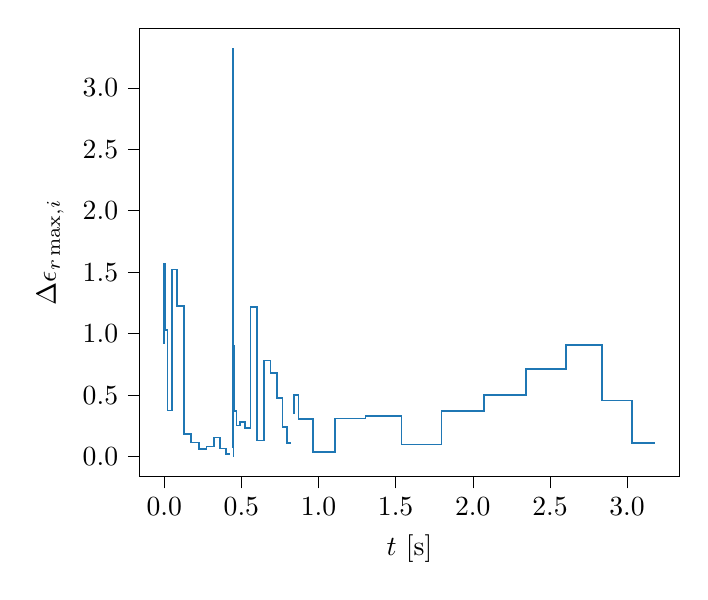
\begin{tikzpicture}

\definecolor{color0}{rgb}{0.12156862745098,0.466666666666667,0.705882352941177}

\begin{axis}[
tick align=outside,
tick pos=left,
unbounded coords=jump,
x grid style={white!69.0196078431373!black},
xlabel={\(\displaystyle t\) [s]},
xmin=-0.158979186761913, xmax=3.33856292200018,
xtick style={color=black},
xtick={-0.5,0,0.5,1,1.5,2,2.5,3,3.5},
xticklabels={
  \(\displaystyle {\ensuremath{-}0.5}\),
  \(\displaystyle {0.0}\),
  \(\displaystyle {0.5}\),
  \(\displaystyle {1.0}\),
  \(\displaystyle {1.5}\),
  \(\displaystyle {2.0}\),
  \(\displaystyle {2.5}\),
  \(\displaystyle {3.0}\),
  \(\displaystyle {3.5}\)
},
y grid style={white!69.0196078431373!black},
ylabel={\(\displaystyle \Delta\epsilon_{r\max,i}\)},
ymin=-0.162644999487379, ymax=3.485119684191,
ytick style={color=black},
ytick={-0.5,0,0.5,1,1.5,2,2.5,3,3.5},
yticklabels={
  \(\displaystyle {\ensuremath{-}0.5}\),
  \(\displaystyle {0.0}\),
  \(\displaystyle {0.5}\),
  \(\displaystyle {1.0}\),
  \(\displaystyle {1.5}\),
  \(\displaystyle {2.0}\),
  \(\displaystyle {2.5}\),
  \(\displaystyle {3.0}\),
  \(\displaystyle {3.5}\)
}
]
\addplot [semithick, color0, const plot mark right]
table {%
0 0.917751320773751
0.0056120056173798 1.56919948623941
0.0221666130741685 1.02951592596602
0.0488337052264625 0.37354458078086
0.0842760827216659 1.52327534115203
0.12671651675769 1.22547758816961
0.174026866756148 0.181644263152705
0.223834794217301 0.114124225981205
0.273642721678455 0.0595710008497272
0.320953071676913 0.0813961626195539
0.363393505712937 0.155882524897358
0.39883588320814 0.0648371947672549
0.425502975360434 0.0190117328490109
0.442057582817223 nan
0.447669588434603 0.57287665548782
0.447694744492815 3.31931219856925
0.447768951264519 2.98605353683469
0.447888487688025 0.303539305891984
0.448047359718729 0.0780418139575947
0.448237600848921 0.189237329105486
0.448449671593784 0.0633921743799786
0.448672937840577 0.00316248613436487
0.44889620408737 0.267013454035912
0.449108274832234 0.0190722256848095
0.449298515962425 0.211014173777279
0.44945738799313 0.0134860711915605
0.449576924416636 0.370097133232656
0.44965113118834 nan
0.449676287246552 0.218457628571746
0.454574962603674 0.90077673609903
0.469025348637549 0.372825637650888
0.492302842652881 0.253149134044869
0.523240213901389 0.279282693428899
0.560286133405463 0.233007358985289
0.60158296407088 1.21939949701796
0.645059910367528 0.129886682187991
0.688536856664177 0.780498384166218
0.729833687329594 0.682351833407182
0.766879606833668 0.477217477838655
0.797816978082176 0.239691223294373
0.821094472097507 0.111497407347172
0.835544858131383 nan
0.840443533488505 0.344466733648252
0.87129471129975 0.498239222952323
0.962301237854726 0.30778513715576
1.10889966590181 0.0381939740121706
1.30373893811699 0.309964463892456
1.53704899981345 0.329334029330994
1.79713071027977 0.0970507592805756
2.0709424865465 0.370016691424663
2.34475426281323 0.499932382683558
2.60483597327954 0.714730349039106
2.838146034976 0.905389318937726
3.03298530719118 0.455102187014554
3.17958373523827 0.110500064622057
};
\end{axis}

\end{tikzpicture}
